% Generated by tex/build_swebok_structure.py from tex/chapters/ch01/10_ソフトウェア要求ツール.tex
\subsubsection{機能テストケース生成ツール}

要求仕様の形式性が高いほど、機能テストケースを機械的に導きやすくなる。たとえば、BDDのシナリオはテストケースへ変換しやすい。状態モデルでは、定義された遷移から正のテストケースを作り、存在しない状態とイベントの組合せから負のテストケースを作れる。

ただし、一般にはツールが入力データを生成できても、期待結果の判断には業務知識が必要になることがある。

\begin{figure}[htbp]
\centering
\IfFileExists{assets/generated_figures/ch01/fig-ch01-12.png}{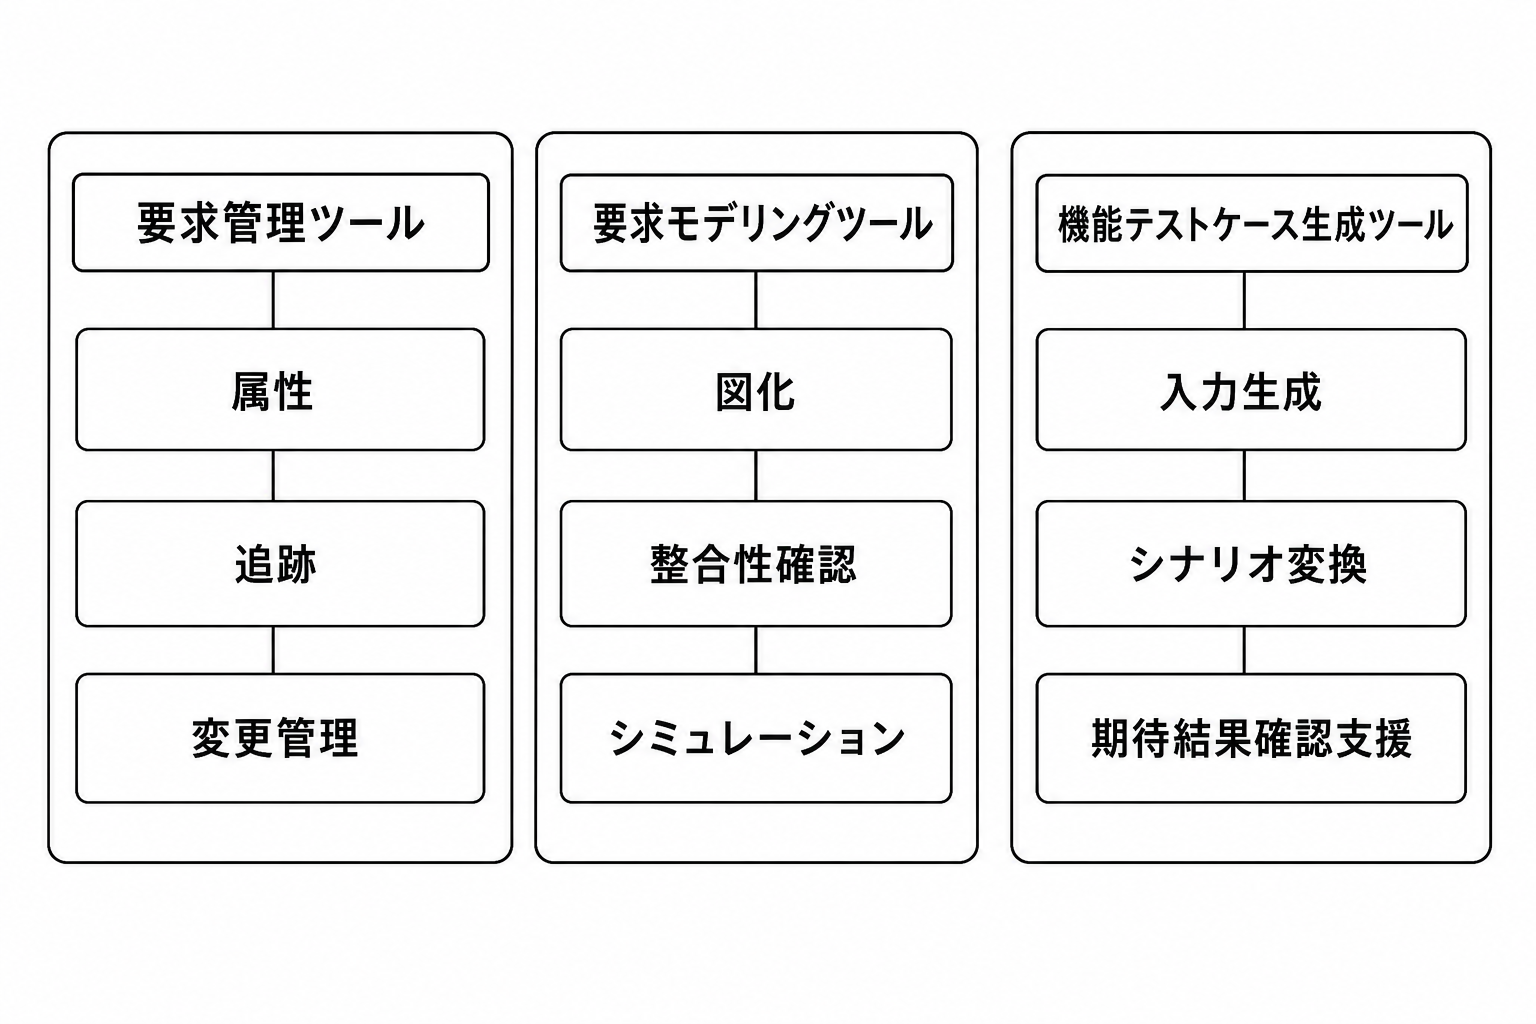
\includegraphics[width=0.96\linewidth]{assets/generated_figures/ch01/fig-ch01-12.png}}{\fbox{\parbox[c][48mm][c]{0.9\linewidth}{\centering 画像生成待ち\\要求ツールの分類図}}}
\caption{要求ツールの分類図}
\label{fig:ch01-12}
\end{figure}
